\documentclass[12pt]{article}

\usepackage[a4paper, total={15cm, 21.5cm}]{geometry}
%\usepackage[italian]{babel}
\usepackage{amsmath}
\usepackage{eurosym}
\usepackage{graphicx}
\usepackage{epsfig}
\usepackage{color}

\newcommand{\be}{\begin{equation}}
\newcommand{\ee}{\end{equation}}
\newcommand{\bea}{\begin{eqnarray}}
\newcommand{\eea}{\end{eqnarray}}

\setlength{\textwidth}{17cm}
\setlength{\oddsidemargin}{-0.5cm}
\setlength{\evensidemargin}{-0.5cm}


\begin{document}


\begin{center}
{\Large\bf Esame di Laboratorio di Fisica Computazionale }\\
{\bf 19 settembre 2017, ore 9.30}
\end{center}



\section{Mathematica}
\begin{enumerate}

\item
  Si definisca una funzione {\tt myFactorial} che prende in input
  un intero $n$ positivo e restituisce il fattoriale $n!$.\\
({\it Si possono usare i comandi nativi di} {\tt Mathematica}
{\it con l'esclusione di} {\tt Factorial} {\it ovvero di} ``!''.)

\item
  Si definisca una funzione {\tt myBinomial} che prende in input
  due interi $n$ e $k$ con $n>k$ e restituisce il coefficiente binomiale
  $\left(\begin{array}{c} n\\k \end{array}  \right)$.\\
({\it Si possono usare i comandi nativi di} {\tt Mathematica}
{\it con l'esclusione di} {\tt Binomial}.)

\item
Si definisca una funzione {\tt myDet3}
che prende in input tre vettori colonna $\vec l_1$, $\vec l_2$ e $\vec l_3$,
ovvero tre liste costituite ciascuna da tre elementi,
e restituisce in output il determinante della matrice
$M\equiv \left( \vec l_1,\, \vec l_2,\, \vec l_3\right)$.\\
({\it Si possono usare i comandi nativi di} {\tt Mathematica}
{\it con l'esclusione di} {\tt Det}.)\\
{\bf Suggerimento:} {\it si utilizzi il comando} {\tt Signature}.


\item
  Si definisca una funzione dei parametri $a$ e $b$ come la soluzione dell'equazione differenziale seguente:
\be
r'(\theta) = b r(\theta),\quad\quad r(0) = a   
\label{eq:eqdiff}
\ee
Si disegni la curva parametrica espressa in coordinate polari dalla coppia
$(r(\theta), \theta)$ al variare del parametro $\theta\in [0,6\pi]$
avendo posto $a=b=1$.


\item
  Si definisca una funzione dei parametri $a$ e $b$ come la soluzione dell'integrale
  \be
p(a,b) \equiv \int_a^b dt\,\frac{1}{\sqrt{(t-a)(b-t)}}
  \ee

  Si disegni in funzione con $a\in [-5,5]$ e con $b\in[-5,5]$
  la superficie $p(a,b)$.
  
\item
Automa cellulare\\[-0.4cm]
\begin{itemize}
\item
Si scriva una funzione che inizializza una lista contenente $2n+1$ elementi, tutti zero con l'eccezione dell'elemento $n+1$, che deve essere posto pari a 1.\\
{\it (Si consideri l'utilizzo combinato di {\tt ReplacePart} e di {\tt Table})}.


\item
Si scriva una lista di regole di sostituzione che realizzi le trasformazioni rappresentate graficamente in figura.\\
{\it (Si consideri per la singola sostituzione una regola del tipo $\{a,b,c\}\to d$)}
\begin{figure}[!h]
\begin{center}
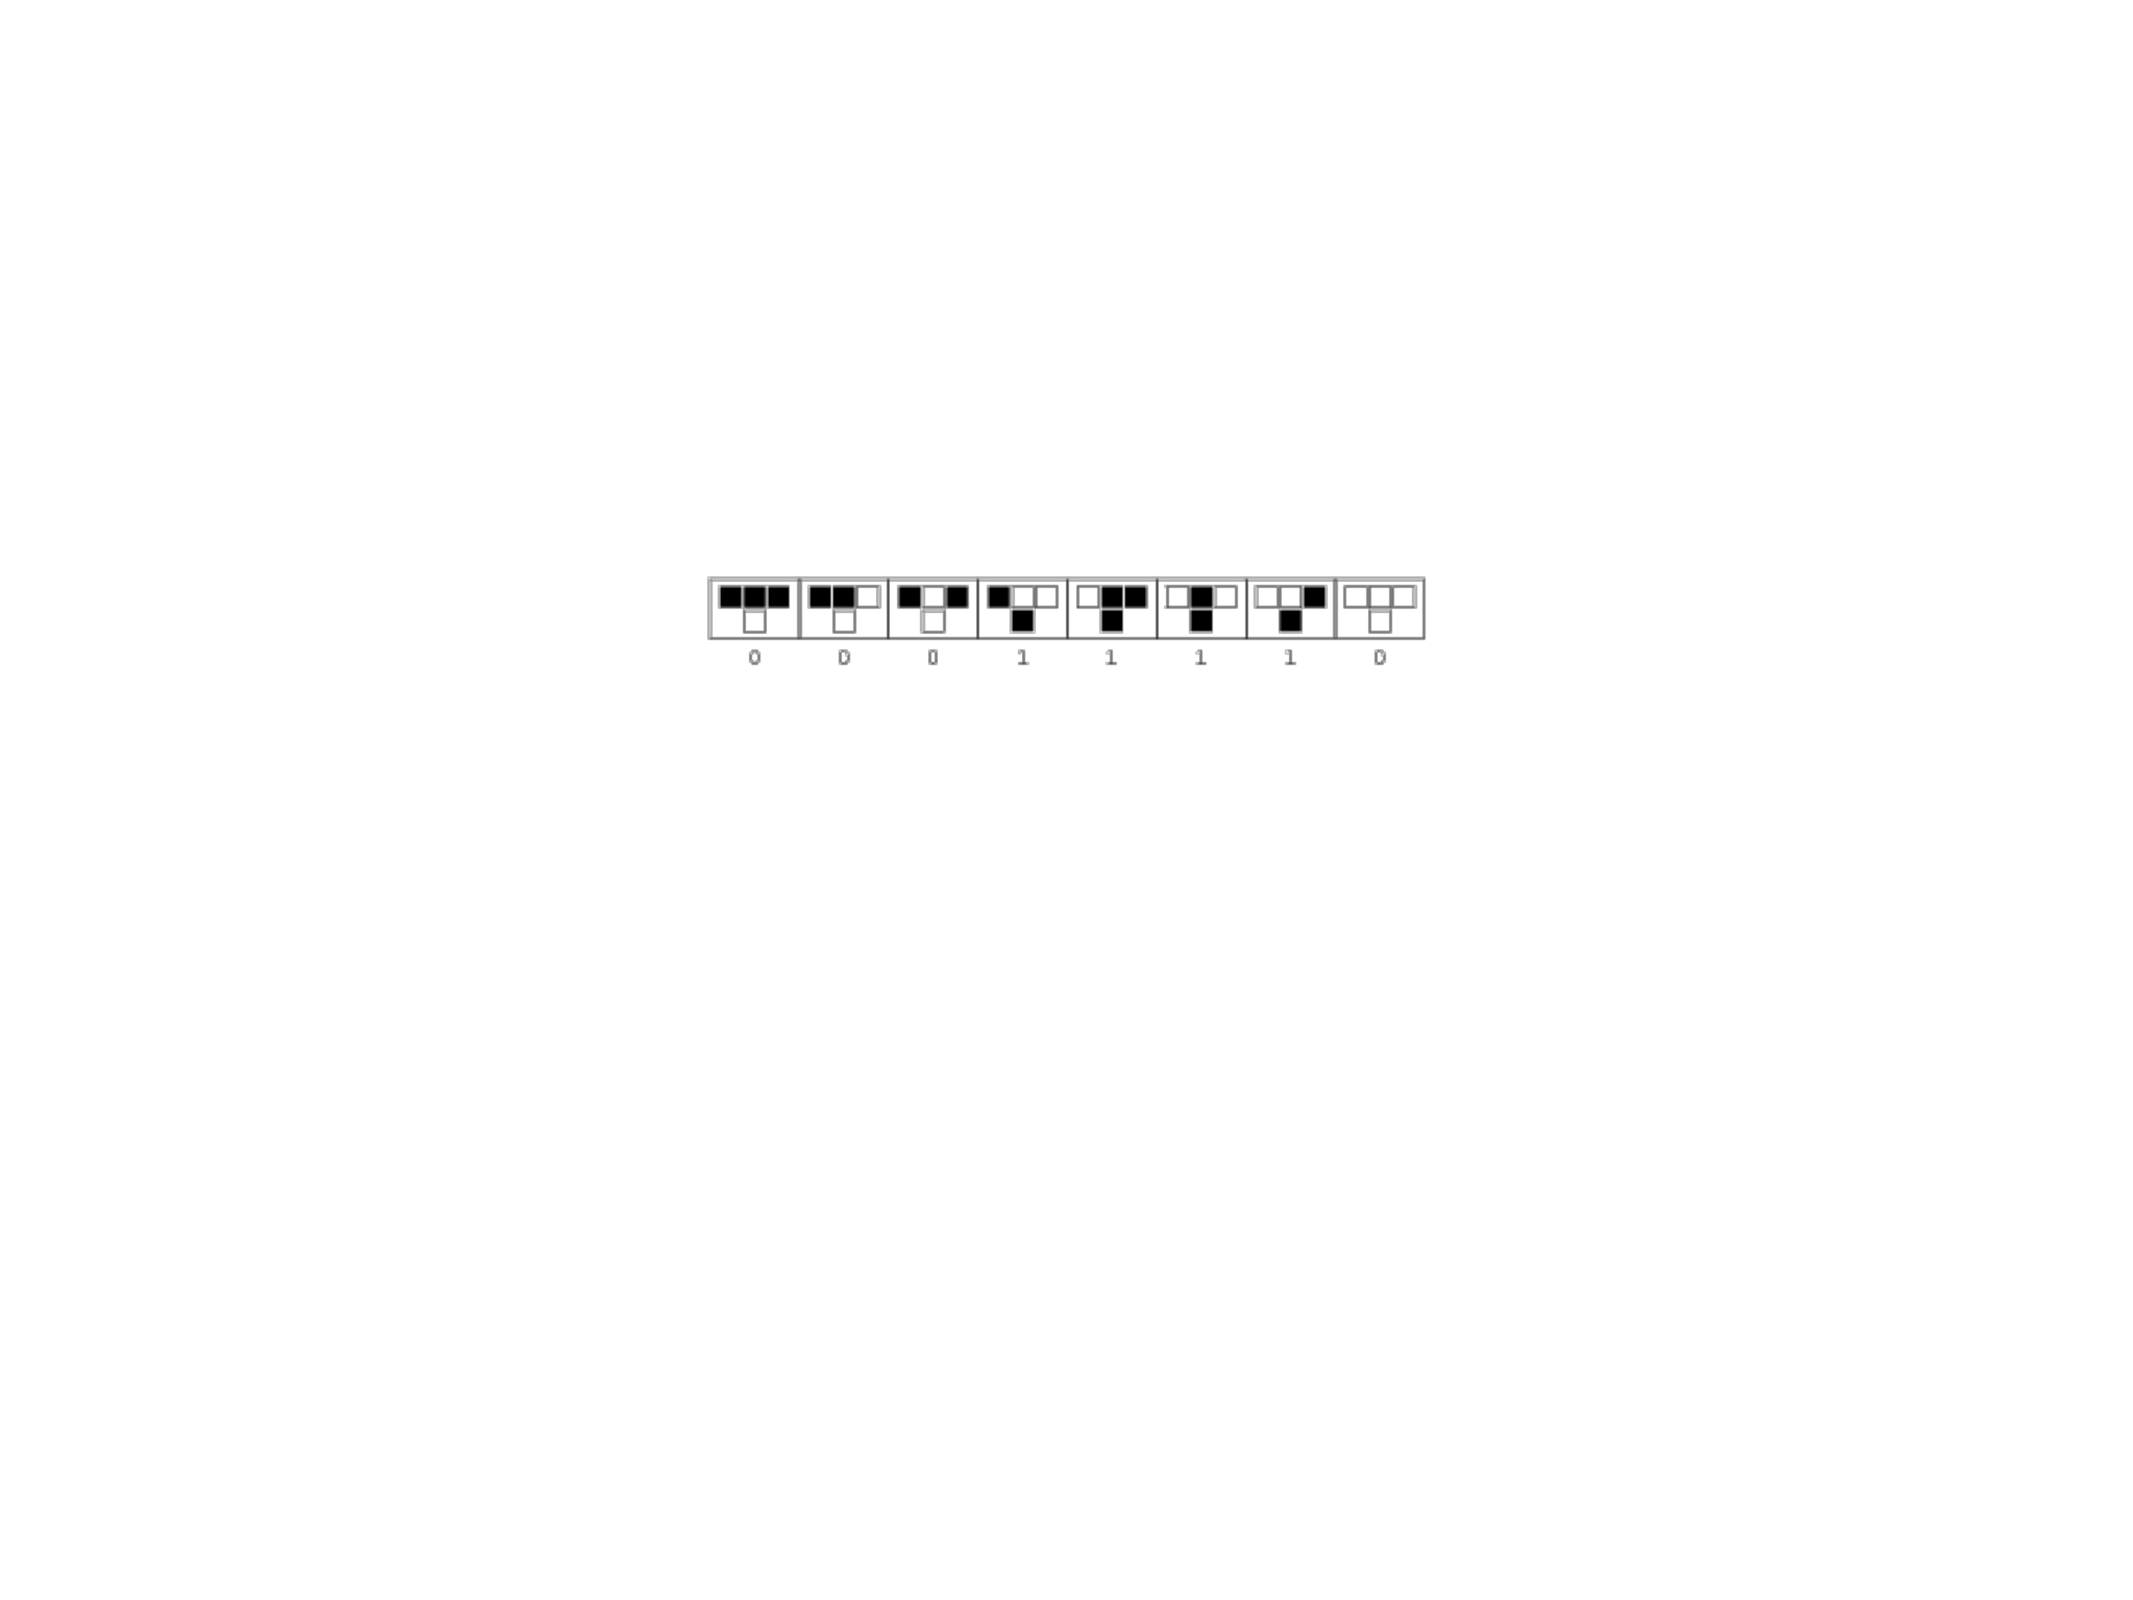
\includegraphics[width=150mm,angle=0]{regola_base.pdf}
\end{center}
\end{figure}

\item
La trasformazione di una lista esistente in una nuova, secondo il meccanismo dell'automa cellulare, richiede di applicare 
a ciascuna terna di elementi consecutivi della lista il set di regole di sostituzione del punto precedente.
Per semplicit\`a, il primo e l'ultimo elemento della lista possono essere ricopiati da una riga all'altra, mentre si devono calcolare tutti gli elementi nuovi dal secondo al penultimo.\\
{\it Si utilizzino i comandi {\tt Table} per generare i nuovi elementi, dal secondo al penultimo, e poi {\tt Prepend} e {\tt Append} per ricopiare il primo e l'ultimo.}

\end{itemize}


\end{enumerate}






\clearpage
\section{C++: Esercizio}



Si risolvano i due esercizi proposti, preferibilmente in due file singoli separati.
La sufficienza \`e raggiunta risolvendo correttamente i primi tre punti del primo esercizio.



\section*{Esercizio 1}


\begin{enumerate}

\item
Si scriva una classe {\tt Vector} che descriver\`a vettori in due dimensioni.
Si pongano come membri privati due variabili {\tt double}, corrispondenti
alle componenti cartesiane del vettore (ad esempio $x$ e $y$).
Si scriva un opportuno costruttore che richieda
come parametri le due coordinate, con valori di default nulli.
Si implementino inoltre due \emph{access function} per leggere le due variabili private.

\item
Si scriva il costruttore di copie (con la sintassi della lista di inizializzazione).
Inoltre si scriva l'operatore ``+='' che esegua la somma con un altro vettore,
e una funzione {\tt theta} che restituisca l'angolo che il vettore forma con l'asse $x$.
[Nota: la funzione {\tt atan} ha valori in $(-\pi/2,\pi/2)$.]

\item
Si scriva la classe {\tt Versor}, derivata di {\tt Vector},
che descriver\`a vettori di norma unitaria.
Si scrivano due costruttori: uno che prenda come parametro l'angolo rispetto all'asse $x$,
e l'altro che prenda un {\tt Vector} e ne costruisca il versore corrispondente.
Bonus se entrambi i costruttori hanno corpo vuoto, cio\`e {\tt \{\}}.

\item
Si scriva l'{\it overriding} dell'operatore ``+='', in modo che sommare un vettore $v$ ad un versore $u$
generi un versore diretto come $u+v$.
Si vuole che questa funzione abbia comportamento polimorfico tra {\tt Vector} e {\tt Versor}.

\item
Si verifichi il comportamento del codice con un {\tt main}
che esegua le seguenti istruzioni:
\begin{itemize}
\item istanziare due vettori $v$ e $w$, inizializzandoli a $(1,1)$ e $(2,2)$ rispettivamente;
\item istanziare un versore $u$, inizializzandolo con $v$;
\item eseguire $u\,+\!=w$;
\item stampare su {\tt std::cout} le componenti di $u$.
\end{itemize}

\item
Per verificare il comportamento polimorfico dell'operatore ``+='',
si ripetano gli stessi passi del punto precedete, utilizzando per\`o tre puntatori
(a $v$, $w$ e $u$), e si controlli che il risultato sia lo stesso.


\end{enumerate}



\section*{Esercizio 2}


Si consideri il tipo {\tt std::vector<int>}
(per comodit\`a lo chiameremo ``Sequenza'';
se si vuole si pu\`o definire un alias con {\tt typedef},
ma non \`e necessario).

\begin{enumerate}

\item
Si scriva una funzione {\tt vsort}, che ordiner\`a in senso crescente gli elementi di
un {\tt std::vector} (passato come argomento) contenente oggetti di tipo Sequenza.
La relazione di ordinamento \`e la seguente: una Sequenza $r$ \`e
minore di $s$ se la somma degli elementi di $r$ \`e minore della somma degli elementi di $s$.
Si usi l'algoritmo {\tt std::sort(it1, it2, pred)}.
Per fare questo sar\`a necessario definire un opportuno predicato {\tt pred},
che confronti due oggetti di tipo Sequenza.
[Si calcoli la somma degli elementi con l'algoritmo {\tt std::accumulate}].

\item
Nel {\tt main}, si istanzi un vettore di sequenze, e vi si inseriscano le due sequenze
{\tt \{3,5,7\}} e {\tt \{1,1,2,3,5\}}.
Lo si ordini e si stampi il terzo elemento della prima sequenza, controllando che sia uguale a 2.

\item
Si scriva una versione {\it generica} della funzione {\tt vsort},
che possa funzionare anche con vettori di sequenze di oggetti di tipo diverso da {\tt int}.
Si controlli, commentando il codice non generico scritto al punto 1, che
il programma funzioni correttamente.

\item
Si renda generico anche il predicato {\tt pred}, con la stessa parametrizzazione descritta al punto precedente.


\end{enumerate}




\clearpage


%%%%%%%%%%%%%%%%%%%%%%%%%%%%%%%%





\section{Shell scripting}

\begin{enumerate}
\item
Si scriva uno script che scambia le due colonne del file {\tt prova.txt} e salva il risultato nel file {\tt scambiate.txt}.
\item
Si scriva uno script che calcola la media dei valori della terza colonna del file {\tt voti.txt}
\item
Si scriva uno script che seleziona, tra tutti i files presenti nella directory
{\tt /home/vicini/corso1617/}, quelli creati nel mese di aprile 2017 e li scrive nel file {\tt aprile.txt}.

\end{enumerate}





\end{document}
